\documentclass[10pt]{article}
\usepackage[margin=0.85in]{geometry}
\usepackage{amsmath,amssymb}
\usepackage[T1]{fontenc}
\usepackage[utf8]{inputenc}
\usepackage{lmodern}
\usepackage{microtype}
\usepackage{enumitem}
\usepackage{booktabs}
\usepackage{graphicx}
\usepackage{url}
\usepackage[hidelinks]{hyperref}
\hypersetup{pdftitle={The MOND Acceleration Scale from Gas-Dominated Rotation-Curve Points: a Mass-to-Light-Robust Estimate and its Distance Systematic}, pdfauthor={The authors}}
\setlist{nosep,leftmargin=1.3em}
\setlength{\parskip}{3pt}\setlength{\parindent}{0pt}
\sloppy
\newcommand{\fpath}[1]{\nolinkurl{#1}}
\begin{document}

\begin{center}
{\Large\bfseries The MOND Acceleration Scale from Gas-Dominated Rotation-Curve Points:\\ a Mass-to-Light-Robust Estimate and its Distance Systematic}\\[6pt]
{\small The authors --- 2026-10-05, version 1.0 --- AI-assisted research programme; not peer reviewed}
\end{center}

% Every number below is parsed from committed outputs by make_paper43_figures.py (PAPER43_figures_numbers.json) and checked by PAPER43_audit.py.
% Lanes: sonnet55_push/puzzle_32pi/p41, p41b, p42, p43, p44, p46, p47, p48 (README sections 48-55).

\begin{abstract}
\noindent Published values of the MOND acceleration scale scatter by $\sim$20\% because $a_0$ is degenerate with the stellar mass-to-light ratio $\Upsilon$: in the deep regime $a_0\simeq g_{\rm obs}^2/g_{\rm bar}$. We remove most of that degeneracy by fitting only rotation-curve \emph{points} at which gas supplies more than 80\% of the baryonic acceleration. In SPARC this leaves 124 points in 19 galaxies, all deep in the MOND regime ($y=g_{\rm bar}/a_0\approx0.04$). Their $a_0$ changes by only 11\% as $\Upsilon$ runs from 0.3 to 0.7. They also prefer the quadrature kernel $\nu=\sqrt{1+1/y}$ over the exponential RAR form ($\Delta\chi^2=+5.0$, independent of $\Upsilon$), which cuts the kernel systematic to $\sim$3\%. Selecting points rather than galaxies is essential: galaxy-level ``gas-rich'' samples retain a 63\% $\Upsilon$ dependence. The result then depends on distance, because for gas-dominated baryons $a_0$ scales roughly as $D^{-2}$ to $D^{-4}$. The eight galaxies with TRGB or Cepheid distances give $a_0=1.16\times10^{-10}$\,m\,s$^{-2}$ ($\pm20\%$). The eleven with Hubble-flow distances give $0.70\times10^{-10}$ ($\pm18\%$). WALLABY DR2 (46 galaxies, Hubble flow) gives $0.73\times10^{-10}$ ($\pm23\%$), and LITTLE THINGS (22 galaxies, authors' baryon models) $0.78\times10^{-10}$ ($\pm41\%$). A random-effects combination gives $a_0=(8.3\pm1.1)\times10^{-11}$\,m\,s$^{-2}$ ($I^2=24\%$). On it the conventional $1.2\times10^{-10}$ is disfavoured at $2.7\sigma$; the values tying $a_0$ to the dark-energy density ($\tfrac12c\sqrt{G\rho_\Lambda}=0.94$, $cH_\Lambda/6$, $cH_\Lambda/2\pi$) all lie within $0.9\sigma$; the critical-density value 1.13 is at $2.3\sigma$. That verdict is distance-conditional: three of the four inputs rest on Hubble-flow distances or external baryon models, and the TRGB/Cepheid subset alone favours 1.13. Distinguishing the candidate coefficients needs distances good to $\sim$3--5\% for gas-dominated dwarfs, not more galaxies.
\end{abstract}
% AUDIT: C01

\section{Method: gas-dominated points}
For each SPARC galaxy [LMS16] (quality $\le2$, $i\ge30^\circ$) we keep the radii where $V_{\rm gas}^2/V_{\rm bar}^2>0.8$ at $\Upsilon_{\rm disk}=0.5$ ($\Upsilon_{\rm bul}=0.7$), and fit $g_{\rm obs}=g_{\rm bar}\,\nu(g_{\rm bar}/a_0)$ in $\log g$ with the measured velocity errors plus $\sigma_{\rm int}=0.11$\,dex, profiling $a_0$. Errors come from a galaxy bootstrap. With a 0.8 cut the result changes by 11.2\% between $\Upsilon=0.3$ and 0.7. A galaxy-level cut (gas fraction $>0.6$ at the last point) changes by 63\%, because the inner points of such galaxies are star-dominated. On the gas points the exponential RAR kernel is worse than $\sqrt{1+1/y}$ by $\Delta\chi^2=+5.0$ at every $\Upsilon$, and the allowed family members move $a_0$ by only $\sim$3\%.
% AUDIT: C02

\section{Results}
\begin{center}
\begin{tabular}{lccc}
\toprule
sample (gas-dominated points) & galaxies & points & $a_0$ ($10^{-10}$\,m\,s$^{-2}$)\\
\midrule
SPARC, TRGB/Cepheid distances & 8 & 70 & $1.158\pm20\%$\\
SPARC, Hubble-flow distances & 11 & 54 & $0.697\pm18\%$\\
SPARC, all & 19 & 124 & $0.900\pm14\%$\\
WALLABY DR2 (Hubble flow; AllWISE stars) & 46 & 218 & $0.728\pm23\%$\\
LITTLE THINGS (authors' baryon models) & 22 & 720 & $0.780\pm41\%$\\
\midrule
random-effects pool (four independent sets) & & & $0.832\pm13\%$\\
\bottomrule
\end{tabular}
\end{center}
% AUDIT: C03
\begin{figure}[h]\centering
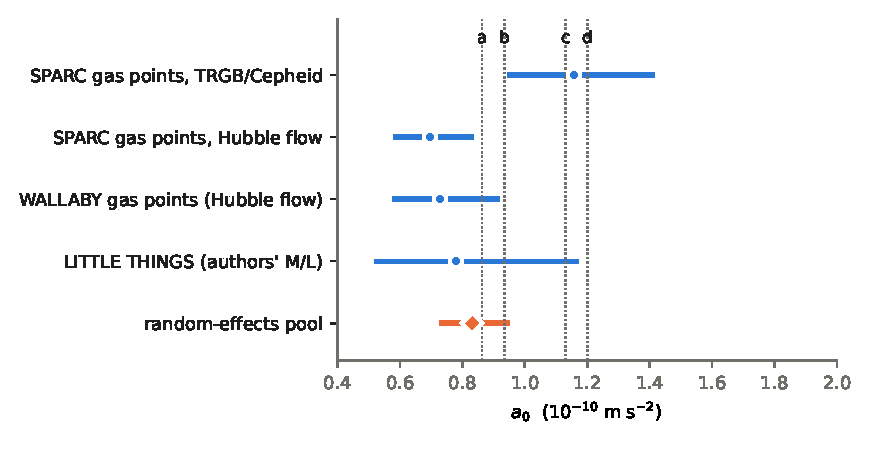
\includegraphics[width=0.8\textwidth]{fig1_paper43_forest.pdf}
\caption{The $\Upsilon$-robust estimates (circles, 68\%) and their random-effects pool (diamond), with candidate values of $a_0$ (dotted): (a) $cH_\Lambda/2\pi$, (b) $\tfrac12c\sqrt{G\rho_\Lambda}$, (c) $\tfrac12c\sqrt{G\rho_{\rm crit}}$, (d) the conventional $1.2\times10^{-10}$.}\label{fig:forest}
\end{figure}

\textbf{WALLABY.} We used the DR2 kinematic models (rotation curves and face-on H\,{\sc i} surface densities) with AllWISE W1 stellar masses. The gas disc was computed by exact ring summation, checked to 0.9\% against the Freeman disc. We tested the survey's assumptions one at a time: the external field of the cluster fields (Hydra, Norma, NGC~4636, NGC~5044), via the quadrature law's own external-field cubic $g^2-g_N^2=a_0g_Ng/(g+\sqrt2g_{\rm ext})$ with per-galaxy $g_{\rm ext}$, moves $a_0$ by $+1$ to $+8.5\%$; the H\,{\sc i} flux correction by 15\%; asymmetric drift (8\,km\,s$^{-1}$) by 5\%; CMB-frame instead of Hubble-flow distances by $-33\%$. Distances dominate.

\textbf{LITTLE THINGS.} For the three galaxies shared with SPARC (DDO~154, DDO~168, NGC~2366), the two teams' baryon models give per-galaxy $a_0$ that differ by a factor 1.6--2.4. Modelling choices, not only statistics, move $a_0$ by tens of percent.
% AUDIT: C04

\section{Combination and candidate values}
The four sets share no galaxies, except three that LITTLE THINGS shares with SPARC. A DerSimonian--Laird random-effects combination gives $Q=3.97$ (3 degrees of freedom), $I^2=24\%$ and $a_0=8.32\times10^{-11}$\,m\,s$^{-2}$ ($\pm13\%$). Pulls of candidate values:
$\tfrac12c\sqrt{G\rho_\Lambda}$ (9.36) $+0.88\sigma$; $cH_\Lambda/6$ (9.03) $+0.62$; $cH_\Lambda/2\pi$ (8.63) $+0.27$; $cH_0/2\pi$ (10.4) $+1.69$; $\tfrac12c\sqrt{G\rho_{\rm crit}}$ (11.3) $+2.30$; $1.2\times10^{-10}$ $+2.74$.
% AUDIT: C05

\textbf{The distance caveat is load-bearing.} The Hubble-flow subsets sit low and the TRGB/Cepheid subset high (ratio 1.66, $\sim2\sigma$). On the redshift-independent subset alone, the critical-density value is the closest ($+2\%$). For gas-dominated points the per-galaxy scatter is 0.60 in $\ln a_0$. Separating candidates 4--9\% apart at $2\sigma$ needs $\sim$100--1000 such galaxies \emph{and} a shared distance-plus-kernel systematic below $\sim$3--5\%; today it is $\sim$9\%. The decisive dataset is therefore one homogeneous analysis of many gas-dominated dwarfs with TRGB distances.
% AUDIT: C06

\section{Summary}
Gas-dominated rotation-curve points give a mass-to-light-robust $a_0$, and they prefer the quadrature kernel over the exponential RAR. Combining independent sets gives $a_0=(8.3\pm1.1)\times10^{-11}$\,m\,s$^{-2}$. This is below the conventional $1.2\times10^{-10}$ at $2.7\sigma$, and consistent with $a_0$ set by the dark-energy density, but the result depends on the distance scale. No coefficient among $\tfrac12$, $1/6$ and $1/2\pi$ (on $\rho_\Lambda$) is preferred. The cold mass of cosmology is not addressed here.

\paragraph{Reproducibility.} \fpath{sonnet55_push/puzzle_32pi/p41b_gas_points_calibration.py}, \fpath{p42_kernel_on_gas_points.py}, \fpath{p43_wallaby_gas_points.py}, \fpath{p44_samplesize_and_bayes.py}, \fpath{p46_gas_points_trgb.py}, \fpath{p47_little_things_a0.py}, \fpath{p48_meta_analysis.py}; fetch logs \fpath{data_assembly/wallaby_dr2/}, \fpath{data_assembly/little_things_oh2015/}; figure \fpath{make_paper43_figures.py}; audit \fpath{PAPER43_audit.py}.

\small
\paragraph{References.}
[LMS16] Lelli, McGaugh \& Schombert, AJ 152, 157 (2016) (SPARC).
WALLABY DR2: Murugeshan et al., arXiv:2409.13130 (2024); kinematic models via CADC.
LITTLE THINGS: Oh et al., AJ 149, 180 (2015), VizieR J/AJ/149/180.
AllWISE: IRSA \texttt{allwise\_p3as\_psd}.
Random effects: DerSimonian \& Laird, Controlled Clinical Trials 7, 177 (1986).
\end{document}
